\documentclass[10pt]{article}
\usepackage[english]{babel}									
\usepackage[utf8]{inputenc}									
\usepackage[T1]{fontenc}										
\usepackage{amsmath,amsfonts,amssymb,amsthm,cancel,siunitx,
calculator,calc,mathtools,empheq,latexsym}
\usepackage{subfig,epsfig,tikz,float}		           
\usepackage{booktabs,multicol,multirow,tabularx,array}        
\usepackage{natbib}
\usepackage{graphicx}
\setlength{\parindent}{0pt}
\setlength{\parskip}{5pt}
\textwidth 13.5cm
\textheight 19.5cm
\columnsep .5cm
\title{\renewcommand{\baselinestretch}{1.17}\normalsize\bf%
\uppercase{<Put Title Here>}
}
\author{
<Put names here>
}


\begin{document}

\date{}

\maketitle

\vspace{-0.5cm}

\begin{center}
{\footnotesize 
<put class name, date, emails, and university affiliation here>
}
\end{center}
\bigskip
\noindent
{\small{\bf ABSTRACT.}
Abstract should concisely
summarize the key findings of the paper. It should consist 
of a single paragraph containing no more than 150 words. 
The Abstract does not have a section number.
}

\medskip
\noindent
{\small{\bf Keywords}{:} 
After the abstract three keywords must be provided.
}

\baselineskip=\normalbaselineskip
% -------------------------------------------------------------------

\section{Introduction and Background}\label{sec:1}
Introduction and background

The study of meteorology and the impact on humans is a multiple century old discipline that includes the study of weather patterns, climate, and many other sub-disciplines. In the modern era, one of the greatest issues in meteorology is the measure of temperature and how it impacts humans that live in different climates. As technology has advanced, systems like air conditioners, heaters, and various home devices that use electricity are more often used than before because of a higher standard of living. Our team with the use of <insert data set name and author> wants to study the relationship between the temperature and human electricity usage in Valencia, Spain and use the results to predict future usage and possible implications of a positive correlation between the two. 

The data set that we chose is generated from ENTSOE, which is a public portal in Spain that collects energy data in the 5 biggest cities in Spain. Since Spain is a large country with a large variability in cities, we compiled a few EDA’s into the many variables that this data set provides such as temperature, pressure, humidity, various forms of electricity generation, total load, etc. Ultimately, the area of greatest interest that we found was Valencia, Spain. Valencia is one of the southern cities that borders the Mediterranean climate and has both a dry and wet climate from the hot summers, to the cool and chilly winters. The variability in temperature, humidity, and electricity usage made Valencia a strong candidate four our case study. 


\section{Literature Review}\label{sec:2}
Logically, we assume that there is a non-linear relationship between the price of electricity and the weather. One assumption that we make is that in the summers, people living in warmer climates are more likely to use air conditioning. In the winters in areas that are cold, there are more likely people that are going to use a heater. In an article by Engle, Granger, Rice, and Weiss titled “Semiparametric Estimates of the Relation between Weather and Electricity Sales”, Engle et al. describe the various factors that affect the relationship between price and weather. The use of a nonparametric regression model is important because it shows how the results are derived from the data and not from predisposed forms/information. Engle et al. review is more comprehensive than the one that our group is taking on as it accounts for many different factors when described, “Estimating this relationship, however, is complicated by the need to control for many other factors such as income, price, and overall levels of economic activity and for other seasonal effects such as vacation periods and holidays” (Engle et al., 310). However, due to the complexity of their model, it is far beyond the scope of our ECS 171 course and cannot easily be replicated. The choice of location they used for their study is St. Louis, a city that experiences both cold weather and warm weather. A summary of their results can be found in Figure 1 below.
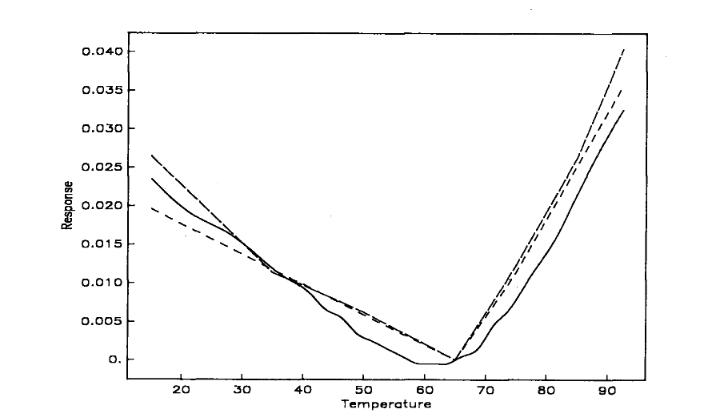
\includegraphics[scale=0.68]{graph1.png}

Figure 1: Engle et al. pg. 316
\\The data shows that there is a positive correlation between the temperature and use in electricity as well as total load. In our experiment we will be measuring exactly these variables but will only use natural occurring phenomena like wind, temperature, and cloud cover. Engle et al. article focused on the percent change, however, our model will focus on the actual correlation between these variables.


\section{Data-set Description and Analysis}\label{sec:3}
Our data-set consists of two CSV files 

\subsection{Case 1}
An example of subsection...

\section{Methodology}\label{sec:4}
For our analysis we utilized several different machine learning methods and algorithms to find which one gave us a possible correlation between variables. Our main methodology was to find a regression model that matched and accurately predicted the outcome of later data. Our group ran many models such as ANN’s, DNN’s, XGBoost, and other various algorithms. 
\\
\\
\textbf{XGBoost}\\
The first model that we found significant success in was the XGBoost regression model. We selected this model due to its widespread adoption in industry applications due to its high model capacity, prediction performance, and other performance benefits such as parallelism (through the implemented framework).  XGBoost is an ensemble model variant, where ensembling occurs in a sequential fashion, using gradient boosting.  Each model in the ensemble is trained to correct the error of the previous model in the ensemble by updating its weights using the gradient of the loss function w.r.t. the previous’ models output (and thus, error).  This allows for computational feasibility and heightened performance.  Further, our data is tabular, a data form that XGBoost handles very well.
\\
\\
<Jaqueline include figure with explanation>

\newpage

\section{Experimental Results}\label{sec:5}

Write all the results here!

\section{Conclusion and Discussion}\label{sec:6}



\bibliographystyle{apalike} 
\bibliography{referencias.bib} 
https://www.tandfonline.com/doi/pdf/10.1080/01621459.1986.10478274?needAccess=true

\end{document}
